\chapter{Design Motivation}
\label{ch:fddp-design}

%%%%%%%%%%%%%%%%%%%%%%%%%%%%%%%%%%%%%%%%%%%%%%%%%%%%%%%%%%%%%%%%%%%%
%\section{Introduction to Dual-Phase Far Detector in DUNE}
\section{Introduction to the DUNE Dual-Phase Far Detector Module Design}
\label{sec:fddp-design-highlight}

%Similarly as for the \single design the \dword{dpmod} is aiming at opening new windows of opportunity in the studyof neutrinos.  DUNE's rich physics program, with discovery potential for \dword{cp} in the neutrino sector, and its capability to make significant observations of nucleon decay and astrophysical events, is enabled by the exquisite resolution of the \lartpc detector technique which is further augmented in the \dual design. The \dual design allows for improving the \dword{s/n} ratio in the charge readout and lowering thresholds for the smallest observable signals while achieving at the same time a finer readout granularity.  The \dual technology aims to build larger drift volumes, thereby reducing %%so 
%the presence of dead materials in the \lar target. The basic physics requirements are identical for both the \single and \dual designs, %%with 
%however, some aspects of the \dual design offer augmented performance. % under some aspects.

The DUNE \dword{dp} \dword{detmodule} aims to open new windows of opportunity in the study of neutrinos, a goal it shares with the \dword{spmod}. 
of neutrinos.  DUNE's rich physics program, with discovery potential for \dword{cp} in the neutrino sector, and its capability to make significant observations of nucleon decay and astrophysical events, is enabled by the exquisite resolution of the \lartpc detector technique, which the \dual design further augments. This design improves the \dword{s/n} ratio in the charge readout,  lowering the threshold for the smallest observable signals while also achieving a finer readout granularity.  The \dual technology enables the construction of larger drift volumes, thereby reducing %so 
the quantity of nonactive materials in the \lar. Although the physics requirements are identical for both the \single and \dual designs, %with 
 some aspects of the \dual design offer augmented performance. % under some aspects.

%%%%%%%%%%%%%%%%%%%%%%%%%%%%%%%%%%%%%%%%%%%%%%%%%%%%%%%%%%%%%%%%%%%%

\section{Dual-Phase (DP) \lartpc Operational Principle}
\label{sec:fddp-operational-principle}

%The basic operational principle is very similar to that of the \single design. %as for the Single-phase design. 
%The precision tracking and calorimetry offered by the \dual
%technology provides excellent capabilities for identifying interactions of interest while mitigating sources of background.  Charged particles traversing the active volume of the \lartpc ionize the medium, while also producing scintillation light.  The ionization \fixme{electron? or charge?} drifts along an \efield that is present throughout the volume, towards a segmented anode.

The basic operational principle is very similar to that of the \single design. 
Charged particles that traverse the active volume of the \lartpc ionize the medium, while also producing scintillation light.  The ionization electrons drift along an \efield towards a segmented anode where they deposit their charge, and \dwords{pd} pick up the scintillation light.
The precision tracking and calorimetry offered by the \dual
technology provides excellent capabilities for identifying interactions of interest while mitigating sources of background.  
Whereas the \single design has multiple drift volumes, the \dword{dpmod} design allows for a single, fully homogeneous \lar volume with a much longer drift length. This volume is surrounded by a \dword{fc} on the sides and a cathode at the bottom, which together define the drift field. 

%The key concept of the \dual design relies on the possibility of amplifying the ionization signal in avalanche processes. In the \single design charges are drifted horizontally to the anode, which consists of a set of induction and collection wire layers immersed in the \lar. In the \dual design electrons are drifted vertically towards an extraction grid just below the liquid-vapor interface. After reaching the grid, the electrons are extracted from the liquid to the gas phase due to an \efield stronger than the drift field. Once in the gas, electrons can be amplified in avalanches that occur in the high-field regions present within micro-pattern gas detectors, the \dwords{lem}. The amplified electrons are then eventually collected on a finely segmented anode with two perpendicular collection views. 

The key differentiating concept of the \dual design is the amplification of the ionization signal in an avalanche process. In the \single design, charges drift horizontally to the anode, which consists of a set of induction and collection wire layers immersed in the \lar. In the \dual design, electrons drift vertically upward towards an extraction grid just below the liquid-vapor interface. After reaching the grid, an \efield stronger than the drift field extracts the electrons from the liquid up into the gas phase. Once in the gas, electrons encounter micro-pattern gas detectors with high-field regions, called \dwords{lem}. The \dwords{lem} amplify the electrons in avalanches that occur in these high-field regions. %The amplified electrons are then collected on a finely segmented anode with two perpendicular collection views. 
The amplified charge is then collected and recorded on a \twod anode
consisting of two sets of \SI{3.125}{mm}-pitch gold-plated copper strips that provide the $x$
and $y$ coordinates (and thus two views) of an event.

%The \dword{dpmod} design allows for  %foresees  a single, fully homogeneous \lar volume with a long drift length. This volume is surrounded (sides and bottom) by a \dword{fc} and a cathode, which together define the drift field. 

%At the top of the \dword{dpmod}, an anode, consisting of a set of active detector elements called \dwords{crp}, sits above the liquid, in the gas phase. The \dwords{crp} integrate the \dwords{lem} and anodes, and support the extraction grid, which is immersed in the liquid. They can be individually positioned at a few millimeters parallel to the interface between the liquid and the gas, ensuring that the extraction grid is immersed.
%The extraction grid, \dword{lem} and anode are assembled into three-layered \textit{sandwiches} with precisely defined inter-stage distances and inter-alignment,  which are then connected together horizontally into

The extraction grid, \dword{lem} and anode are assembled into three-layered \textit{sandwiches} 
with precisely defined inter-stage distances and inter-alignment,  which are then connected together horizontally into
modular units of area \num{9}~m$^2$. These units are called \dwords{crp}.
The \dwords{crp} integrate the \dwords{lem} and anodes, and support the extraction grid. These units can be individually positioned in a horizontal plane a few millimeters beneath the liquid-gas interface, ensuring complete immersion of the extraction grid. 

The argon scintillation light, which at a wavelength of  \SI{128}{nm} is deep in the UV spectrum and it is recorded by an array of \dwords{pmt} located below the cathode.  %The \dwords{pmt} are coated with a material that shifts the wavelength closer to the visible spectrum and subsequently record the time and pulse characteristics of the incident light.
The \dwords{pmt}, coated with a wavelength-shifting material, shifts the light  closer to the visible spectrum and records the time and pulse characteristics of the incident light.

%The performance of the  \lartpc hinges on several key factors.  First, the purity of the \lar must be extremely high in order to allow the ionization to be able  to drift over several meters towards the anode planes.  The levels of electronegative contaminants (e.g., oxygen, water), must be reduced andmaintained to $\sim$ppt levels in order to achieve minimum charge attenuation over the longest drift lengths in the \lartpc.  The \dual and \single designs are subject to the same purity requirements. Second, the electronic readoutof the \lartpc requires very low noise levels so that the signal from the drifting ionization  is clearly discernible over the baseline of the electronics.  %%The \dual design relies on the same purity requirements as for Single-Phase and on the use of low noise cryogenic electronics. However the impact of these aspects on the performance is mitigated by the possibility of amplifying the electrons signal in the gas phase. On the other hand the \dual design requires higher voltages to be applied to the cathode in order to define the drift field over longer paths.
%This requires use of low-noise cryogenic electronics. However the impact of these aspects on the performance is mitigated by the possibility of amplifying the electrons signal in the gas phase. On the other hand the \dual design requires higher voltages to be applied to the cathode in order to define the drift field over longer paths.

Two key factors affect the performance of the  \lartpc{}.  First, the \lar purity must be extremely high in order to achieve minimum charge attenuation over the longest drift lengths in the \lartpc{}.  This requires that the levels of electronegative contaminants (e.g., oxygen, water), be reduced and
maintained at $\sim$ppt levels.  The \dual and \single designs are subject to the same purity requirements. 
%
Second, the electronic readout
of the \lartpc{} requires very low noise levels in order that the signal from the drifting electrons
%\fixme{charge} 
be clearly discernible over the baseline of the electronics.  This requires use of low-noise cryogenic electronics. 

The amplification of the electron signal in the gas phase mitigates the potential impact of these factors on the performance of the \dual design.  On the other hand this design requires  higher voltages on the cathode, relative to the \single, due to the longer drift field. 


\begin{dunefigure}[Principle of the \dual readout]{fig:figure-label-DPprinciple}{Principle of the \dual readout}
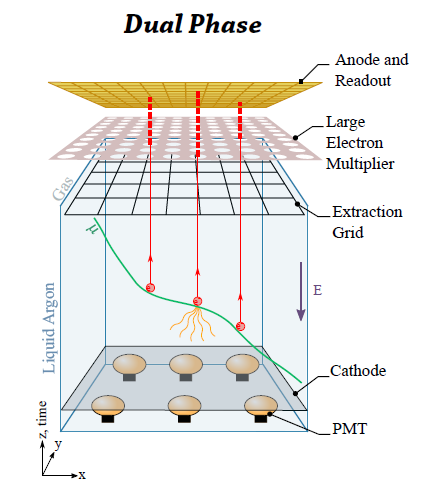
\includegraphics[width=0.8\textwidth]{dualphase-principle}
\end{dunefigure}

%%%%%%%%%%%%%%%%%%%%%%%%%%%%%%%%%%%%%%%%%%%%%%%%%%%%%%%%%%%%%%%%%%%%
\section{Motivation for the \dual Design} % at DUNE}
\label{sec:fddp-design-motivation}

%The innovative \dual design is similar in many ways to the \single design, but implements some unique features and offers several advantages over it, in particular the electron amplification in the gas phase that enables a robust and tunable \dword{s/n} ratio.  The features of the \dual design, e.g., high gain,  allow achieving very long drift paths, compensating for losses due to electronegative impurities, and large detector dimensions while minimizing the number of readout channels, thanks to the long projective geometry.  In addition a \dword{dpmod} is built out of a smaller number of construction modules and readout channels than an equivalent \dword{spmod}. The \dual detector design provides other practical advantages such as the full accessibility to all the \dword{fe} electronics which can be replaced at any time while the detector is operating without contaminating the \lar volume. All these aspects, providing an appealing and complementary approach to the Single-Phase design, as summarized below:

The innovative \dual design is similar in many ways to the \single design, but implements some unique features and offers several advantages over it, providing an appealing and complementary approach, as summarized below:

%\fixme{I found the paragraph and the list very redundant. I think the (modified) list covers everything (anne)}

\begin{itemize}
\item Gain on the ionization signal obtained in the gas phase:
\begin{itemize}
\item  leading to a robust and tunable \dword{s/n} and a lower detection threshold, and
\item  compensating for potential charge attenuation due to long drift paths; 
\end{itemize}
\item  Larger fiducial volume, enabling very long drift paths;
\item  Absence of dead material in the \lar drift volume;
\item  Finer readout pitch (\SI{3}{mm}), implemented in two identical collection views, $x$ and $y$;
\item  Fewer readout channels (\dpnumcrpch for \dual versus \spnumch for \single for a  \nominalmodsize module); 
\item  Fewer construction modules;
\item  Full accessibility and replaceability of the \dword{fe} electronics during the detector operation.

\end{itemize}

 The \dual design features maximize the capability of the experiment and are motivated to cope with the unprecedented scale of the \dwords{detmodule} and the deep underground location where construction will occur.

Among the features driven by the underground location of the experiment, all detector components are sized to fit within the constraints of the \surf shafts and access pathways. The \dword{crp} modules are essentially planar objects with a surface of \num{3}\,$\times$\,\SI{3}{m$^2$}. All the other detector %modules 
components (\dword{fc} and cathode modules) are %as well 
designed in order to stay within this envelope. The relatively small number of detector elements makes the underground installation easier.

A drift time of several milliseconds is typical for ionization charge to arrive at the anode wires after drifting several meters.  This lengthy duration, as well as aspects of the DUNE physics program looking for rare and low-energy processes, makes the deep underground location essential for the \dword{dpmod}.  The \SI{1.5}{km} overburden of earth will vastly reduce the rate of cosmic rays reaching the active volume of the \dword{dpmod}, greatly enhancing the ability to search for rare and low-energy signatures without the influence of cosmic-induced backgrounds.  

%\fixme{Not sure this last pgraph needs to be here - should be in intro volume (anne)}






%%%%%%%%%%%%%%%%%%%%%%%%%%%%%%%%%%%%%%%%%%%%%%%%%%%%%%%%%%%%%%%%%%%%
\section{Overview of Dual-Phase Design}
\label{sec:fddp-ov-description}

This \dual design implements a \dual liquid argon time projection chamber (\lartpc) augmented with a light-readout system.  \textit{\dual} refers to the extraction of ionization electrons at the interface between the liquid and gas argon and their amplification and collection in the gas phase.

The \dword{dpmod} features a  \dpactivelarmass active mass \lartpc, with all associated cryogenics, electronic readout, computing, and safety systems. The \dword{dpmod} is designed to maximize the active volume within the confines of the membrane cryostat while minimizing dead regions and the presence of dead materials in the drift region. The detector is built as a single active volume \dptpclen long, \dptpcwdth wide and \tpcheight high, with the anode at the top, the cathode near the bottom, and an array of \dwords{pmt} located  at the bottom %of the vessel 
underneath the cathode. The active volume (see Figure~\ref{fig:DPdet1}) is surrounded by the \dword{fc}. The ionization electrons in the liquid phase drift  in a uniform \efield towards the anode plane at the top of the active volume. This is made by an array of \num{80} independent \dword{crp} modules, \num{3}\,$\times$\,\SI{3}{m$^2$} each. The cryogenic \dword{fe} electronics is %hosted 
installed in the \dwords{sftchimney}
% signal penetrations (chimneys)
on the roof of the cryostat. There are no active electronics elements in the cryostat volume besides the \dword{pmt} bases.
The proposed design optimally exploits the cryostat volume of \cryostatwdth{}(w)\,$\times$\,\cryostatht{}(h)\,$\times$\cryostatlen{}(l) with an anode active area of \dptpcwdth{}\,$\times$\,\cryostatlen{} and a maximum drift length of \dpmaxdrift{}, corresponding to an active \lar mass of \dpactivelarmass  (\dpfidlarmass fiducial). 

The detector elements (\dwords{crp}, \dword{fc} and cathode) have been modularized such that their production can proceed in parallel with the construction of the DUNE caverns and cryostats, and sized so that they conform to the access restrictions for transport underground. Table~\ref{tab:dune-dp-parameters} summarizes %some of 
the high-level parameters of the \dword{dpmod} while Figure~\ref{fig:DPdet1} shows %an overview of the \dword{dpmod}  with its main components.
the \dword{dpmod}'s main components.

\begin{dunetable}[Dual-phase module parameters]{lll}{tab:dune-dp-parameters}{\Dword{dpmod} parameters}
Parameter & Value & Note \\ \toprowrule
Cryostat \lar Mass & \larmass & \\ \colhline 
Active \lar Mass & \dpactivelarmass & \\  \colhline 
Active height & \tpcheight & \\  \colhline 
Active length & \dptpclen & \\  \colhline 
Maximum drift & \dpmaxdrift & \\ \colhline 
Number of \dwords{crp} &\dptotcrp & \\  \colhline 
Number of \dword{crp} channels & \dpnumcrpch & \\ \colhline 
Number of \dword{pmt} channels & \dpnumpmtch & \\ 
\end{dunetable}

% %% % %
\begin{dunefigure}[Diagram of the \dword{dpmod}]{fig:DPdet1}
  {The \dword{dpmod} with cathode, \dwords{pmt}, \dword{fc} and anode plane with \dwords{sftchimney}.}
%  {The \dword{dpmod} with cathode, \dwords{pmt}, \dword{fc} and anode
%    plane with \dword{sft} \dword{chimney}.}
  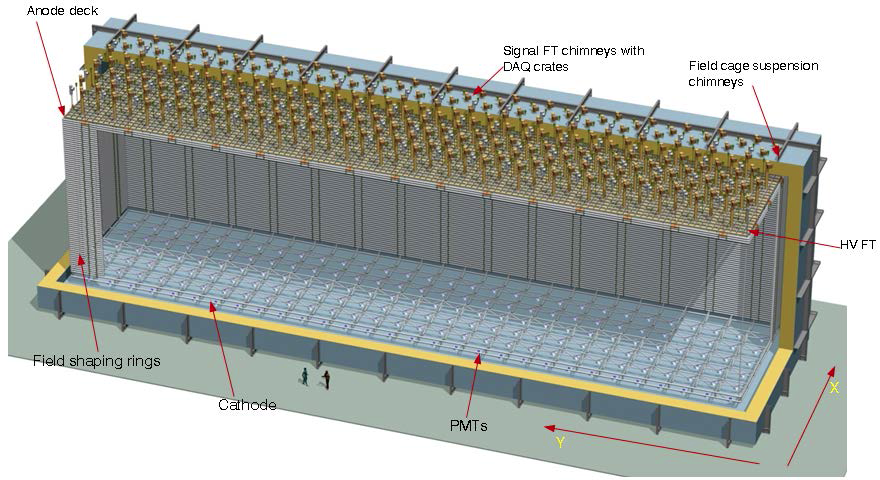
\includegraphics[width=0.9\textwidth]{DUNE-CDR-detectors-volume-optim.png}
\end{dunefigure}

The extraction of the electrons from the liquid to vapor phase is performed thanks to the submersed horizontal extraction grid, integrated in each \dword{crp} structure. A \dword{crp} unit includes \dpswchpercrp (0.5~m$\times$0.5~m) \dword{lem}/anode sandwiches, providing tunable amplification and charge collection on two independent views organized in strips of \SI{3}{m} length and \dpstrippitch pitch. There are \dpchpercrp readout channels for each \dword{crp}. Signals in each \dword{crp} unit are collected via three \dwords{sftchimney}
% fdth{} chimney
hosting the \dword{fe} cards with the cryogenic \dword{asic} amplifiers (\dpchperchimney channels/chimney) which are accessible and replaceable without contaminating the pure \lar volume. Each \dword{sftchimney} is coupled to a microTCA crate ensuring the signals' digitization and 
\dword{daq}. These crates are connected  via optical fiber links to the \dword{daq} back-end. The total number of readout channels  per \nominalmodsize module is \dpnumcrpch.

Each \dword{crp} unit is independently suspended by three stainless steel ropes. The vertical level of each \dword{crp} unit can be automatically adjusted with respect to the \lar level via three suspension \fdth{}s. The stainless steel ropes are operated by step motors located outside the suspension \fdth{}s. Slow-control \fdth{}s,  one per \dword{crp} unit, are used for level meters and temperature probes readout,
%\fixme{used for level meter and temperature probe readout?}
  for pulsing the calibration signals, and to apply the \dword{hv} bias on the two sides of the \dwords{lem} and on the extraction grid. The \dword{fc} and the anode are constructed of modules of similar dimensions as those in \dword{pddp}.

The number of components and corresponding parameters for the \dpactivelarmass \dword{dpmod} are summarized in Table~\ref{tab:DP_numbers}.

\begin{dunetable}[Quantities of items or parameters for the \dword{dpmod}]{ll}{tab:DP_numbers}{Quantities of items or parameters for the \dpactivelarmass  \dword{dpmod}}  Item & Number or Parameter    \\ \toprowrule
Anode plane size & W = \dptpcwdth, L = \dptpclen \\ \colhline
\dword{crp} unit size & W = \SI{3}{m}, L = \SI{3}{m}  \\ \colhline
\dword{crp} units & \num{4}\,$\times$\,\num{20} = \dptotcrp \\ \colhline
\dword{lem}-anode sandwiches per \dword{crp} unit & \dpswchpercrp \\ \colhline 
\dword{lem}-anode sandwiches (total) & \dpnumswch \\ \colhline
\dword{sftchimney} per \dword{crp} unit & \num{3} \\ \colhline
\dword{sftchimney} (total) & \num{240} \\ \colhline
Charge readout channels / \dword{sftchimney} & \num{640}  \\ \colhline
Charge readout channels (total) & \dpnumcrpch \\ \colhline
Suspension \fdth per \dword{crp} unit & \num{3}  \\ \colhline
Suspension \fdth{}s (total) & \num{240}  \\ \colhline
Slow Control \fdth per sub-anode & \num{1}  \\ \colhline
Slow Control \fdth{}s (total) & \num{80} \\ \colhline
\dword{hv} \fdth & \num{1}  \\ \colhline
\dword{hv} for vertical drift & \dptargetdriftvoltpos \\ \colhline
Voltage degrader resistive chains & \num{12} \\ \colhline
%Cathode modules & \dpnumfcres  \\ \colhline
Cathode modules & \num{80}  \\ \colhline
%Field cage rings & \dpnumfcrings     \\ \colhline
Field cage rings & \num{197}     \\ \colhline
%Field cage ring vertical spacing & \SI{200}{mm}  \\ \colhline
%Field cage resistors (total) & \dpnumfcres    \\ \colhline
%Field cage modules & \dpnumfcmod  \\ \colhline
Field cage modules (\SI{3}{m}$\times$\SI{12}{m}) & \num{48}  \\ \colhline
\dwords{pmt} (total) & \dpnumpmtch (\num{1}/m$^2$) \\ 
\end{dunetable}



A number of factors make the \dual TPC concept, as described in this chapter, well suited to large detector sizes like the \dword{dpmod}.
In this design,the charge amplification in the \dwords{crp} compensates for the charge attenuation on the long drift paths.  This configuration also simplifies
construction by optimally exploiting the long vertical dimensions of the cryostat, providing a large homogeneous fiducial volume  free of embedded passive materials (effectively increasing the detector size), reducing the number of readout channels,  and ultimately lowering costs.  


The \dwords{crp} collect the charge in a projective way,  with practically no dead region, and read the signals out  in two collection views, eliminating the need for  induction views, 
which  simplifies the reconstruction of complicated topologies. The tunable high \dword{s/n} provides operative margins with respect to the noise and electron lifetime conditions, and lowers the threshold on the minimal  detectable energy depositions .

The scope of a \dword{dpmod} includes the design, procurement, fabrication, testing, delivery, installation and
commissioning of the detector components, which is organized in detector consortia, specific to \dual or joint with \single. %DP consortia or joint \single{}-\dual consortia):

\begin{itemize}
\item \dword{crp}, including extraction grid, \dword{lem} and anode and readout planes (\dual consortium);
\item Analog and digital electronics and \dword{sftchimney} (\dual consortium); 
\item \dword{pds} (\dual Consortium);
\item Cathode, \dword{fc} and \dword{hv} system (joint \single{}-\dual consortium);  
\item Slow-control (joint \single{}-\dual consortium); 
\item Back-end \dword{daq} system (joint \single{}-\dual consortium).
\end{itemize}


%%%%%%%%%%%%%%%%%%%%%%%%%%%%%%%%%%%%%%%%%%%%%%%%%%%%%%%%%%%%%%%%%%%%%%
\section{Detector systems}
\label{sec:fddp-ov-systems}
%%%%%%%%%%%%%%%%%%%%%%%%%%%%%%%%%%%
\subsection{Charge Readout Planes}
\label{v4:fddp-ov:crp}

An extraction efficiency of \num{100}\,\% of the electrons from the liquid to the gas phase is achieved with an \efield of the order of \SI{2}{kV/cm} across the liquid-gas interface, applied between an  extraction grid submersed in the liquid and charge amplification  devices situated in the ultra-pure argon gas. 

These amplification devices, called \dwords{lem}, are horizontally  oriented \SI{1}{mm}-thick printed  circuit boards with electrodes on the top and bottom surfaces. They are drilled through with many holes that collectively form a micro-pattern structure;  when a \SI{3}{kV} potential difference is applied across the electrodes the ionization electrons are amplified by avalanches (Townsend multiplication) occurring in the  pure argon gas in this micro-pattern structure due to the high \efield (\SI{30}{kV/cm}).

The use of avalanches to amplify the charges in the gas phase increases the \dword{s/n} ratio by at least one order of magnitude with a  gain between \numrange{20}{100}, significantly improving the event reconstruction quality. It also lowers the threshold for small energy depositions and provides a better resolution per volumetric pixel (voxel) compared to a \single \lartpc.  The charge is collected in a finely segmented \twod ($x$ and $y$) readout anode plane at the top of the gas volume and fed to the \dword{fe} electronics.   

The  collection, amplification and readout components are combined in an array of independent (layered) modules called \dwords{crp}. A \dword{crp} is  composed of several \num{0.5}\,$\times$\,\SI{0.5}{m$^2$} units, each of which is composed  of a \dword{lem}-anode \textit{sandwich}.  These units are embedded in a mechanically reinforced frame of FR-4 and iron-nickel invar alloy. This design guarantees the planarity requirements over the \dword{crp} span although the temperature gradient present in the gas phase and possible sagging effects with respect to the three suspension points. The \dword{crp} structure also integrates  the submersed extraction grid, which is an array of $x$ and $y$ oriented stainless steel wires, \SI{0.1}{mm} in diameter, with \dpstrippitch pitch. Thicknesses and possible biasing voltages for the different layers are indicated in Figure~\ref{fig:CRP_struct}.

\begin{dunefigure}[Thicknesses and HV values for electron extraction from liquid to gaseous Ar]{fig:CRP_struct}
{Thicknesses and \dword{hv} values for electron extraction from liquid to gaseous argon, their  multiplication by \dwords{lem} and their collection on the $x$ and $y$ readout anode plane. The \dword{hv} values are indicated for a drift field of \SI{0.5}{kV/cm} in \lar.}
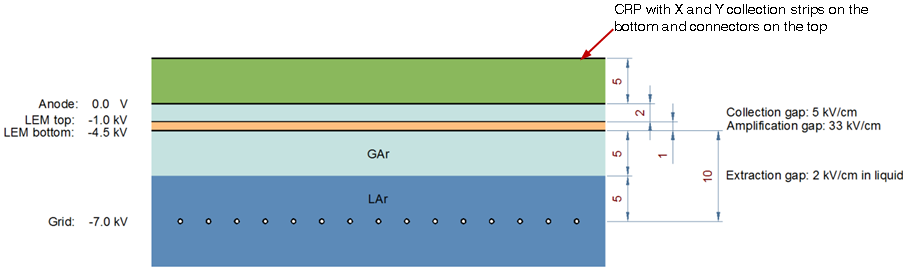
\includegraphics[width=0.8\textwidth]{CRP_gaps.png}
\end{dunefigure}

Each \dword{crp} is independently suspended by three stainless-steel ropes linked to the top deck of the cryostat. This suspension system allows adjustment of the \dword{crp} distance and parallelism with respect to the \lar surface, and keeps the extraction grid immersed. A \dword{crp} provides an adjustable charge gain (with a minimal required gain of \num{20}) and two independent, orthogonal readout views, each with a pitch of \dpstrippitch.  The \dword{lem}/anode sandwiches  in the same \dword{crp} unit are interconnected with short flat cables so that each readout channel corresponds to a total strip length of \SI{3}{m}. Combined with the time information coming from the \lar scintillation readout by the \dword{pmt} arrays ($t_0$), a \dword{crp} provides \threed track imaging with $dE/dx$ information.  The \dwords{crp} and their components are described in Chapter~\ref{ch:fddp-CRP}.

The typical amplification achieved by this design, between \numrange{20}{100}, improves the \dword{s/n} ratio and thus  compensates for the charge losses that occur along the very long drift paths due to the presence of  electronegative impurities. Therefore, despite the longer drift length, this design requires no higher 
purity of the \lar than does the reference design, around \SI{0.1}{ppb} (or \SI{100}{ppt}) of oxygen equivalent, and yields a \SI{3}{ms} electron lifetime. The required level of purity can be reached by starting from  commercially available ppm-level bulk argon and filling a non-evacuated vessel~\cite{WA105_TDR}.

%The \dword{s/n} ratio can exceed \num{100} for a \dword{mip} after a drift path of %12~m
% \dpmaxdrift (given an electron lifetime of \SI{3}{ms}, a drift field of \SI{0.5}{kV/cm} and a \dword{lem} gain of \num{180}). With the same drift field, the same electron-lifetime conditions and a \dword{lem} gain of \num{25}, the \dword{s/n} is larger than \num{50}:\num{1} for tracks up to \SI{6}{m} from the anode; it reaches \num{14}:\num{1} for \dword{mip} tracks that are \dpmaxdrift from the anode.

For instance, given an electron lifetime of \SI{3}{ms} corresponding to the minimal requirement,  a drift field of \SI{0.5}{kV/cm} and a \dword{lem} gain of \num{20}, \dword{s/n} ratio would be larger than  \num{40}:\num{1} for tracks up to \SI{6}{m} from the anode, while reaching  \num{11}:\num{1} for  \dword{mip} tracks that are \dpmaxdrift from the anode.


Other \fdth{}s than the signal chimney connected to the \dwords{crp} and the \dword{crp} slow control and \fdth{}s are planned for the cathode \dword{hv} connection, the \dwords{crp}' suspension and level adjustment, the \dword{hv} and signal readout of the \dwords{pmt}, and the monitoring instrumentation (level meters, temperature probes, strain gauges, etc.).

%%%%%%%%%%%%%%%%%%%%%%%%%%%%%%%%%%%
\subsection{Readout Electronics and Chimneys}
\label{v4:fddp-ov:electronics}

The electrical signals from the collected charges are passed to the outside of the tank via a set of dedicated \dword{sftchimney}. The chimney are pipes passing through the top layer of the cryostat insulation and closed at the top and at the bottom by ultra-high-vacuum flanges (warm and cold). The volume inside each \dword{sftchimney} is tight with respect to the cryostat inner volume and it is filled with nitrogen gas. The bottom (cold) flange of each \dword{sftchimney} is a short distance %with respect to 
from the \dwords{crp} in the cryostat gas volume.

The cryogenic \dword{fe} electronics cards, housed at the bottom of the chimney are plugged to the top side of  the cold flange. The \dword{fe} cards are based on analog cryogenic preamplifiers implemented in \dword{cmos} \dword{asic} circuits for high integration and large-scale affordable production. 
The \dword{asic} circuits have been especially designed, following an R\&D process started in 2006, to match the signal dynamics of a \dword{dpmod}. Within the chimney, the cards are actively cooled to a temperature of about \SI{110}{K} and isolated with respect to the \lar vessel by the cold flange \fdth{}.  The bottom side of the cold flange is connected to the \dword{crp} via short flat cables (of length \SI{0.5}{m}) in order to minimize the input capacitance to the preamplifiers. Each \dword{sftchimney} collects \num{640} readout channels. 

%The \dword{sftchimney} design allows access to and replacement of the analog \dword{fe} electronics from the outside without contaminating the \lar volume since the \dword{fe} cards are mounted on \SI{2}{m} long blades that slide on lateral guides that are integrated into the mechanical structure of the chimney. 

The \dword{fe} cards are mounted on \SI{2}{m} long blades that slide on lateral guides that are integrated into the mechanical structure of the chimney, allowing access to and replacement of the analog \dword{fe} electronics from the outside without contaminating the \lar volume. 
Swapping the \dword{fe} electronics requires opening a flange at the top of the \dword{sftchimney} and feeding the \dword{sftchimney} with nitrogen in slight over-pressure with respect to the atmospheric pressure.  This operation quite rapid and straightforward, and can be performed while the \dword{detmodule} is taking data. The chimney act also as Faraday cages, thereby entirely decoupling the analog \dword{fe} electronics %with respect to 
from possible noise pickup from the digital electronics.   

%The digital electronics for the  charge digitization system is located at warm on the roof the cryostat. This layout makes possible the use of low cost/high speed  networking technologies used in the telecommunication industries such as microTCA. The digital electronics was also developed thanks to a long R\&D process started in 2006.  Digitization cards in the microTCA  Advanced Mezzanine Card (\dword{amc}) format read 64 channels/card. Each \dword{amc} card can digitize all the 64 channels at 2.5 MHz and compress and transmit this continuous data stream, without zero skipping, over a network link operating at 10 Gbit/s. Lossless data compression is particularly effective thanks to the high S/R of \dual which limits noise contributions at the level of 1 ADC count. Each signal \dword{sftchimney} is coupled to a \dword{utca} crate housing in 10 \dword{amc} digitization cards in order to read 640 channels and transmit the data via the  microTCA Carrier Hub (\dword{mch}) switch via a 10 Gbit/s optical link connected to the \dword{daq} back-end. 240 \dword{utca} crates are sufficient to read the entire detector module. The \dword{sftchimney} warm flange is used to connect the analog differential signals, via shielded VHDCI cables, to the \dword{amc} digitization cards and also to distribute the low voltage and slow control signals to the analog \dword{fe} electronics.  

The digital electronics for the charge digitization system, also resulting from a long R\&D process started in 2006, is located %at warm 
on the roof the cryostat at room temperature. This makes it possible to use the low-cost, high-speed  networking technologies used in the telecommunication industries, such as \dword{utca}. 
Digitization cards in the \dword{amc} format read \num{64} channels per card. Each \dword{amc} card can digitize all  \num{64} channels at \SI{2.5}{MHz} and compress and transmit this continuous data stream, without zero skipping, over a network link operating at \SI{10}{Gbit/s}. Lossless data compression is particularly effective thanks to the high S/N ratio
%\fixme{S/N?} yes
 of \dual{}, which limits noise contributions at the level of one \dword{adc} count. Each \dword{sftchimney} is coupled to a \dword{utca} crate housing in \num{10} \dword{amc} digitization cards in order to read  \num{640} channels and transmit the data via the \dword{mch} switch via a \SI{10}{Gbit/s} optical link connected to the \dword{daq} back-end. It requires \num{240} \dword{utca} crates to read the entire \dword{detmodule}. The \dword{sftchimney} warm flange is used to connect the analog differential signals, via shielded VHDCI cables, to the \dword{amc} digitization cards and also to distribute the \dword{lv} and slow control signals to the analog \dword{fe} electronics.  

The light-readout digitization system is also based on \dword{utca} \dword{amc} cards derived from the design of the charge readout and hosting a specific circuitry, based on the CATIROC \dword{asic} for the light-readout triggering. By assuming a \dword{pmt} channel density similar to that in \dword{pddp}, five \dword{utca} crates are sufficient to read \dpnumpmtch \dwords{pmt}.

The timing synchronization is based on the \dword{wr} standard. Specifically developed timing \dword{mch} connected to a \dword{wr} network ensure the distribution of clock, absolute timing, and trigger information on the backplane of the \dword{utca} crates. The \dword{wrmch} are connected via \SI{1}{Gbit/s} optical fibers to a system of \dword{wr} switches which interconnect the \dword{wr} network. This ensures that the digitization performed by the various \dword{amc} cards is completely aligned and it also refers to the absolute UTC time. 
%\fixme{...ensures...  that it connects to the absolute...?}
The \dword{wrgm} switch is connected to a GPS disciplined oscillator unit providing absolute time and the clock frequency reference to the system. The timing system includes \num{16} \dword{wr} switches and \num{240} (charge readout) + \num{5} (light readout) \dword{mch} units.    

%The entire readout electronics system has been optimized in order to cope to the \dual features including charge signals dynamics, the readout organization via the chimney, the number of readout channels, the high \dword{s/n} ratio and the possibility of performing a continuous data streaming with zero losses to the \dword{daq} back-end. The other aspect which has been taken into account since the beginning of the R\&D is the costs reductions and optimization by using particularly cost effective technologies and by performing the corresponding developments in order to fully exploit these technologies.  This optimization adds to the fact that the number of readout channels is naturally lower for a \dword{dpmod} thanks to the long projective geometry: \dpnumcrpch channels for a DP module with 3 mm readout pitch to be compared to \spnumch channels for a \single module with 5 mm readout pitch.

The entire readout electronics system has been optimized to support the \dual features including: charge signal dynamics, readout organization via the chimney, the number of readout channels, the high \dword{s/n} ratio, and the possibility of performing continuous data streaming with zero losses to the \dword{daq} back-end. 

%Also taken into account since the beginning of the R\&D are cost reduction and optimization. Employing cost-effective technologies and performing the corresponding R\&D needed to fully exploit these technologies.  

Employing cost-effective technologies and performing the corresponding R\&D needed to fully exploit these technologies are strategies that are in place since the beginning of the R\&D period in order reduce and optimize costs.   
This optimization adds to the fact that the number of readout channels is naturally lower for a \dword{dpmod} thanks to the long projective geometry: \dpnumcrpch channels for a DP module with 3 mm readout pitch to be compared to \spnumch channels for a \single module with 5 mm readout pitch. %

%\fixme{This must be the 3rd time I've read this information! Can we remove last sentence?} No, costs optimization is an important point to stress

%%%%%%%%%%%%%%%%%%%%%%%%%%%%%%%%%%%
\subsection{Cathode, Field Cage and HV System}
\label{v4:fddp-ov:cathode}

The \dword{hv} system is designed by a common \single{}-\dual consortium.
The drift field (E ${\simeq}$ \SI{0.5}{kV/cm}) inside the fully active \lar volume is produced by applying \dword{hv} to the cathode plane at the bottom of the cryostat and is kept uniform by the \dword{fc}, a stack of \num{60} equally spaced field-shaping electrodes,  polarized at linearly decreasing voltages from the cathode  voltage to almost ground potential, reached at the level of the \dword{crp}. The electrodes are rectangles made of extruded aluminum profiles (vertical pitch \SI{60.6}{mm}) with rounded corners running horizontally (and stacked vertically) around the active volume. The aluminum profiles are supported and insulated by FRP supporting beams with a pattern of slots where the aluminum profiles can be mounted. Similarly as in \dword{pddp} the profiles are arranged in modules of \SI{3}{m} width including two FRP supporting columns. These modules are chained together and  are hanging from the cryostat roof. A chain of \num{6} modules covers the \dpmaxdrift drift. The aluminum profiles of the different modules are joined together with short clipping profiles in order to ensure the electrical continuity over the
%\fixme{specific?}  in order to ensure the electrical continuity of the %60 m 
\dptpclen long horizontal rings. 

%\fixme{this just refers to one leg of the rectangle, right?  Arent they 2x60 + 2x12 m long?} Yes

The drift cage design shares common structure elements (aluminum profiles and FRP supporting beams) as the \single \dword{fc} design but with a different arrangement (vertically hung structure) in order to cope with the \dword{dpmod} geometry.

The cathode structure, constructed of a reinforced frame to guarantee its planarity, is suspended from the \dword{fc} and hangs near the 
bottom of the cryostat. It is a segmented structure of tubes of different sizes  arranged in a grid to minimize weight, limit sagging and avoid high \efield
regions in its proximity.  The segmented structure allows scintillation light to pass through and be detected by uniform arrays of \dwords{pmt} mounted \SI{1}{m} below it at the bottom of the tank. As in \dword{pddp}, the cathode is made out of modules \SI{3}{m} in size in order to allow for transportation and underground installation. 

%%%%%%%%%%%%%%%%%%%%%%%%%%%%%%%%%%%
\subsection{Photon Detection System}
\label{v4:fddp-ov:pd}

The \dword{pds} is based on an array of \dwords{pmt} uniformly distributed below the cathode. Assuming a similar channel density as in \dword{pddp}, this translates to \dpnumpmtch channels. The \dwords{pmt} have a \dword{tpb} coating on the photocathode's external glass surface that shifts the scintillation light from deep UV to visible light. The \dwords{pmt}  sit on the corrugated membrane cryostat floor, on %thanks to specific 
mechanical supports that do not interfere with the membrane thermal contraction. %Each \dwords{pmt} is connected via a single \dword{hv} cable which allows at the same time for \dword{hv} biasing and signals transmission thanks to a positively biased base circuity. This allows for limiting the number of \fdth{} channels.
A single \dword{hv} cable provides both \dword{hv} biasing and signal transmission to each \dword{pmt} by way of a positively biased base circuity, thus reducing the required number of \fdth{} channels.
A system of optical fibers provides for the \dwords{pmt} calibration.  


%%%%%%%%%%%%%%%%%%%%%%%%%%%%%%%%%%%
\subsection{Data Acquisition}
\label{v4:fddp-ov:daq}

The Ethernet-based \dword{daq} back-end system is designed by a joint \single{}-\dual consortium. It connects to %the 
\SI{10}{Gbits/s} optical links that provide continuous, lossless, compressed data streaming from the \dword{utca} crates, and it has the task of determining the trigger conditions for \textit{interesting} events (beam, cosmics, \dword{snb} neutrino interactions). This system also manages the recording of data to disk. % and of organizing the writing of the related data on disk. 
The system can exploit the high \dword{s/n} ratio peculiar to the \dual design, the availability of the entire data stream without losses, and the possibility of going to lower detection thresholds for \dword{snb} events.

 It  is assumed that this \dword{daq} back-end system will be composed of a set of event-building and trigger machines, high-performance network elements, and a high-bandwidth distributed storage system based on an array of storage servers operating in parallel. In particular, the \dword{daq} system is expected to:

\begin{itemize}
\item Collect the high-bandwidth data volume coming from the data links of the \dword{fe} digitization crates; 
\item Put together the data streams from different crates in Regions Of Interest (ROI) or over the entire detector volume (A ROI is typically the size of a \dword{pddp} four-\dword{crp} surface, since events are contained in such a region.);
\item Process this data flow by an online trigger farm %in order to 
as a prelude to selecting relevant events to be recorded on disk (both neutrino beam and off-beam events);
\item Produce charge-readout triggers independently of the light-readout triggers and beam-spill information %In particular, triggers over a sliding timing window of about \SI{10}{s} may be issued by the trigger farm for the search of SN neutrinos based on the presence of low energy depositions, in order to dump on disk the entire content of the SN trigger sliding time window
(In particular for \dword{snb} events, the trigger farm would issue triggers over a sliding timing window of about \SI{10}{s}  based on the presence of low-energy depositions; the entire content would be dumped to disk.).
\end{itemize}

%The \dual readout architecture can be organized organized in 20 ROI, each similar to the \dword{pddp} back-end architecture. Triggers are searched on the level 1 event builder machines, interconnecting multiple \dword{utca} crates, on a sliding windows of 10 s contained in the event builder RAM memory.
%The event builders combine the continuous lossless-compressed data streaming from the charge readout with beam data and with light data in order to define the window T0 and select disk streams from beam events, cosmics and SNa events. The data decompression in necessary on the event builders in order to perform the charge data analysis while compressed are kept in memory for further writing on disk from level 2 machines of the output streams: beam, cosmics/proton decay, SNa neutrino burst. The level 1 events builders exchange trigger primitive data on the network with a global supervisor machine which then decides for the data writing on disk. The supervisor can order the dump on disk of the event builders memory  windows if a certain number of candidate energy depositions is found from the charge data. It is possible to put in communication in this scheme also parts of different 10 kton modules
%For beam data and cosmic events typically the amount of data written on disk can be limited to one or two ROI in case events are not contained in a single ROI but happen at the border in between two ROI. 

The \dual readout architecture can be organized organized into \num{20} \dwords{roi}, each similar to the \dword{pddp} back-end architecture. Triggers are searched on the level-1 event builder machines, interconnecting multiple \dword{utca} crates, on a sliding windows of \SI{10}{s}  contained in the event builder RAM. % memory.

%\fixme{I'm not sure how to parse prev sentence (anne)}

The event builders combine the continuous lossless, compressed data (streaming from the charge readout) with beam data and light data in order to define the window $t_0$ and select disk streams from beam events, cosmics and \dword{snb} events. The data decompression is necessary on the event builders in order to perform the charge data analysis for the triggers definition. Compressed data are kept in memory, while the trigger definition analysis is performed, for further writing on disk from level-2 machines from the output streams: beam, cosmics and proton decay, and \dword{snb}. 
%\fixme{check prev sentences; they were garbled and I fixed. Anne} done
The level-1 event builders exchange trigger primitive data on the network with a global supervisor machine, which then decides what data to write onto disk.  The supervisor can order the dump onto disk of the event builder's memory  windows if a certain number of candidate energy depositions is found from the charge data. 
This scheme makes it possible to put selected portions of different \dwords{detmodule} in communication with one another.  
Typically for beam data and cosmic events, the amount of data written to disk can be limited to one or two \dwords{roi}; there are cases in which in case events occur at the border between two \dwords{roi} rather than in a single one.


%%%%%%%%%%%%%%%%%%%%%%%%%%%%%%%%%%%
\subsection{Cryogenics Instrumentation and Slow Controls}
\label{v4:fddp-ov:sc}
The \dword{cisc} system is designed by a joint \single{}-\dual consortium. %The slow control system has to deal with the readout of the following items
This system controls the % biasing of the \dword{hv} for the \dwords{lem}s and \dwords{crp}, and manages the 
following items:

\begin{itemize}
\item Cryogenic instrumentation: measurements of temperatures (gas and liquid), pressure (gas), liquid level, purity monitors;
\item \dword{crp} instrumentation: temperatures, pulsing system, precision level meters, readout of \dword{crp} stepping motors;
\item Generation and control of \dword{hv} biasing of \dword{lem} and grid;
\item Generation and control of \dword{hv} biasing for the \dwords{pmt} and calibration (via optical pulsing);
\item Slow control of the \dword{utca} crates, analog \dword{fe}\dword{lv} control, charge injection control to preamplifiers;
\item Control of the cathode \dword{hv} biasing system;
\item Alignment survey of \dword{crp} position (via external reference points);
\item Control of the laser system;
\item Analysis of \lar purity and \dword{lem}  gain calibration.
\end{itemize}
